\documentclass{IEEEtran}
\usepackage[spanish]{babel}
\usepackage[utf8]{inputenc}
\usepackage{blindtext}
\usepackage{amsmath}
\usepackage{graphicx}
\title{Proyecto de Investigación Aplicado a Algo Interesante}
\author{Gerardo M. Chávez-Campos}
\begin{document}
\maketitle
\section{Introducción}
\blindtext[2]
\section{Materiales y métodos}
En \eqref{fourier} siguiente se muestra la 
transformada de Fourier.
\begin{equation}
    f(x)=\int_0^{\infty}x sin(\omega)\label{fourier}
\end{equation}
En \eqref{recta} se muestra la formula para ....
\begin{equation}
    y=mx+b\label{recta}
\end{equation}

\blindtext[8]
\section{Resultados}
\blindtext[4]
\begin{figure}
    \centering
    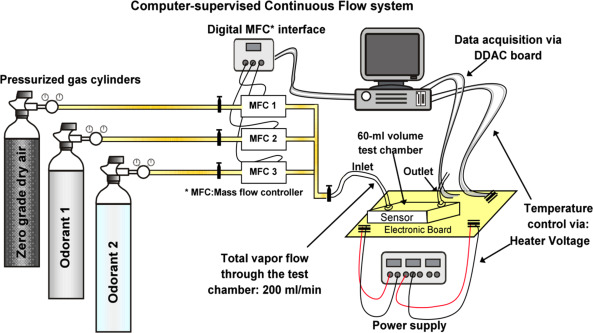
\includegraphics[width=2.5in]{metodologia.jpg}
    \caption{Caption}
    \label{fig:my_label}
\end{figure}








\section{Conclusiones}
\blindtext[1]
\end{document}

